\section{Model}
\label{sec:model}

In this section, we first formulate the machine comprehension problem and then describe the model. We adopt the following terminology. Let $N$ be the length of the context and $M$ be the length of the question. $D$ is the embedding size and $H$ is the hidden size of the model.


\subsection{Problem Statement}
\label{subsec:problemstatement}

The machine comprehension task considered in this paper is as follows. Given a context paragraph with N words C = \{$c_1$, $c_2$, ..., $c_N$\} and a query sentence with M words Q = \{$q_1$, $q_2$, ... $q_M$\} output a span S = \{$c_i$, $c_{i+1}$,...${c_{i+j}}$\} from the original paragraph C. 

\begin{table}[htbp]
    \caption{An example of a machine comprehension task.}
    \label{table:economicSchools} 
    \centering
    \begin{tabular}{|l|p{0.8\linewidth}|}
    \hline
    Question   &  Economy, Energy and Tourism is one of the what? \tabularnewline \hline
    Context  & Subject Committees are established at the beginning of each parliamentary session, and again the members on each committee reflect the balance of parties across Parliament. Typically each committee corresponds with one (or more) of the departments (or ministries) of the Scottish Government. The \textcolor{blue}{current Subject Committees} in the fourth Session are: Economy, Energy and Tourism; Education and Culture; Health and Sport; Justice; Local Government and Regeneration; Rural Affairs, Climate Change and Environment; Welfare Reform; and Infrastructure and Capital Investment \tabularnewline \hline
    Answer   & current Subject Committees \tabularnewline \hline
    \end{tabular}
 
\end{table}

\subsection{Model Overview}
\label{subsec:models}

Several state-of-the-art machine comprehension models have a similar structure. They have an embedding layer, an embedding encoder layer, a context-query attention layer, a model encoder layer and an output layer. We introduce two novel extensions to this structure.  One, we add a Embedding Attention Layer as a form of self-attention over the embedding layer and show that it indeed improves model performance. Second, for the embedding encoder layer we use a combination of recurrent and convolution operations. 

Thus, our machine comprehension model is a hierarchical multi-stage process consisting of six layers. 

\begin{enumerate}
\item \textbf{Embedding Layer}. This layer is a mix of character embedding and word embeddings. 
\item \textbf{Embedding Attention Layer}
\item \textbf{Embedding Encoder Layer}
\item \textbf{Attention Flow Layer}
\item \textbf{Model Encoder Layer} blah blah
\item \textbf{Output Layer} blah blah
\end{enumerate}

The details of each of the layers are as follows.

\paragraph{1. Embedding Layer.} In this layer we mix character embeddings with word embeddings. 

For character embeddings, we use a method similar to that proposed by Kim et al \cite{kim2016character}. We first convert a word to its character indices. We then pad (or truncate) each word so it has length $m_{word}$.  For each of these characters we lookup a dense character embedding (which has shape ${e_{char}}$). To combine the character embeddings, we use 1-dimensional convolutions over $m_{word}$ using ${e_{char}}$ as the input channel size. The output of the CNN are max-pooled over the entire width to obtain a fixed-size vector of shape ${e_{word}}$ for each word. 

For word embeddings, we use pre-trained word vectors from GloVe \cite{} to obtain the fixed embedding for each word. The size of the word embeddings is ${e_{word}}$ which is the same as the shape of the character-level embeddings for each word.  


\paragraph{2. Embedding Attention Layer.} Several state-of-the-art machine comprehension models have a similar structure. They have an embedding layer, an embedding encoder layer, a context-query attention layer, a model encoder layer and an output layer. We introduce two novel extensions to this structure.  One, we add a `Base Attention Layer` as a form of self-attention over the embedding layer and show that it indeed improves model performance. Second, for the embedding encoder layer we use a combination of recurrent and convolution operations. 

\paragraph{3. Embedding Encoder Layer.} Several state-of-the-art machine comprehension models have a similar structure. They have an embedding layer, an embedding encoder layer, a context-query attention layer, a model encoder layer and an output layer. We introduce two novel extensions to this structure.  One, we add a `Base Attention Layer` as a form of self-attention over the embedding layer and show that it indeed improves model performance. Second, for the embedding encoder layer we use a combination of recurrent and convolution operations. 

\paragraph{4. Attention Flow Layer.} Several state-of-the-art machine comprehension models have a similar structure. They have an embedding layer, an embedding encoder layer, a context-query attention layer, a model encoder layer and an output layer. We introduce two novel extensions to this structure.  One, we add a `Base Attention Layer` as a form of self-attention over the embedding layer and show that it indeed improves model performance. Second, for the embedding encoder layer we use a combination of recurrent and convolution operations. 

\paragraph{5. Model Encoder Layer.} Several state-of-the-art machine comprehension models have a similar structure. They have an embedding layer, an embedding encoder layer, a context-query attention layer, a model encoder layer and an output layer. We introduce two novel extensions to this structure.  One, we add a `Base Attention Layer` as a form of self-attention over the embedding layer and show that it indeed improves model performance. Second, for the embedding encoder layer we use a combination of recurrent and convolution operations. 

\paragraph{6. Output Layer.} Several state-of-the-art machine comprehension models have a similar structure. They have an embedding layer, an embedding encoder layer, a context-query attention layer, a model encoder layer and an output layer. We introduce two novel extensions to this structure.  One, we add a `Base Attention Layer` as a form of self-attention over the embedding layer and show that it indeed improves model performance. Second, for the embedding encoder layer we use a combination of recurrent and convolution operations. 

\begin{figure*}[h!]
\centering
	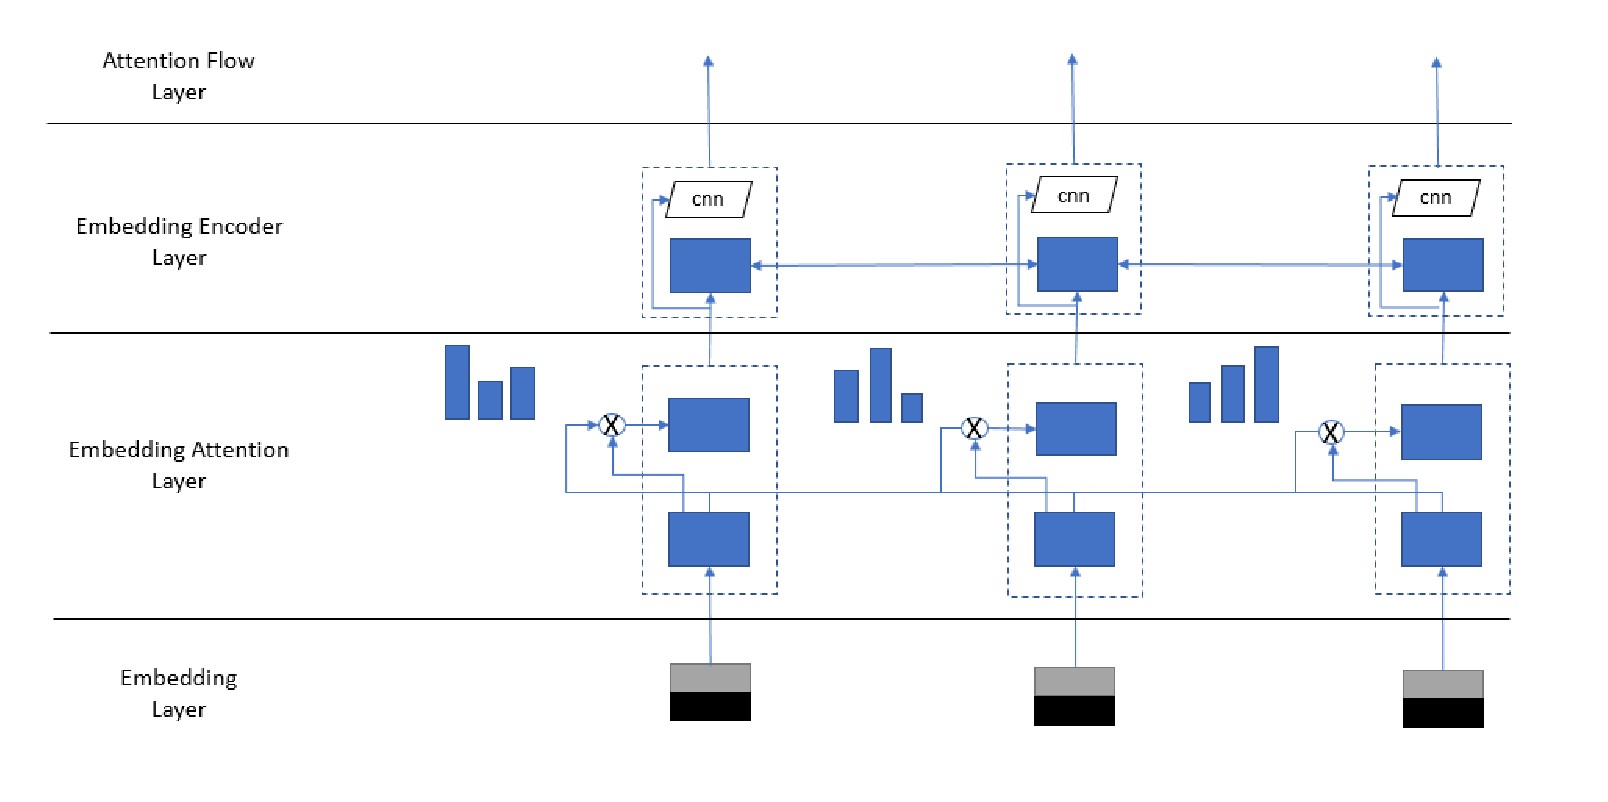
\includegraphics[width=12cm]{Figs4Paper/ModifiedLayers.eps}
  \caption{Convolutional network architecture}
  \label{fig:convnetarchitecture}
\end{figure*}

%\begin{figure*}[h!]
%\centering
	%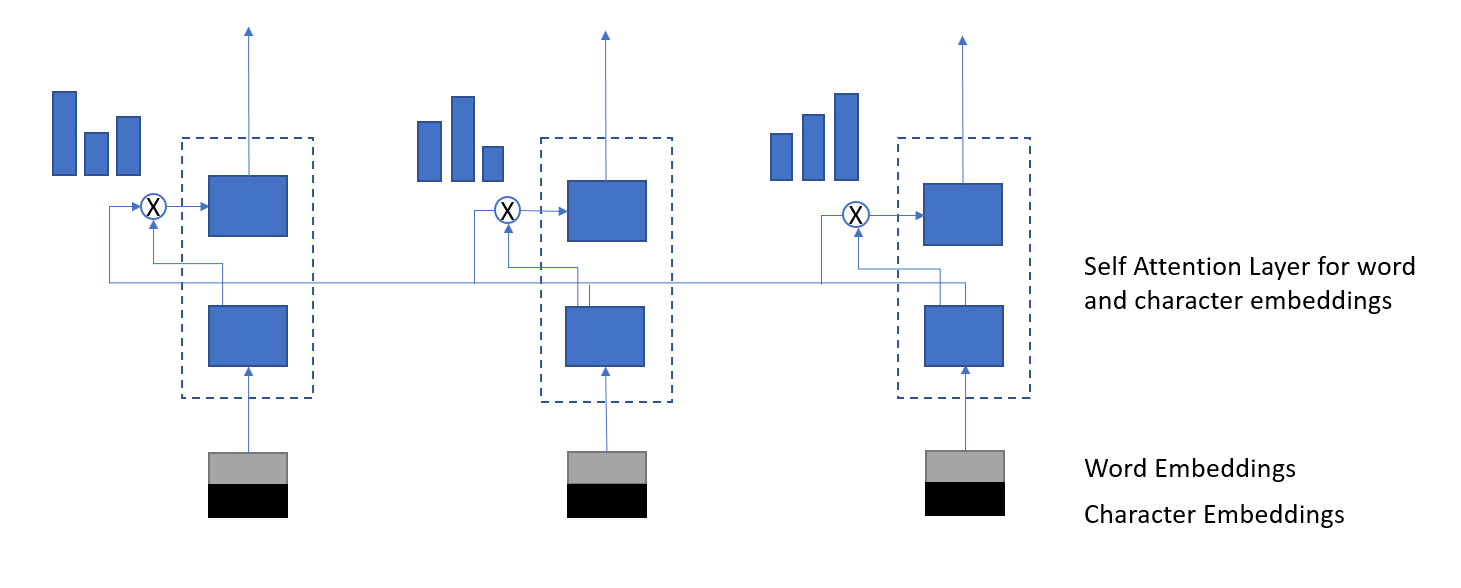
\includegraphics[width=12cm]{Figs4Paper/EarlyAttentionLayer.eps}
  %\caption{Convolutional network architecture}
  %\label{fig:convnetarchitecture}
%\end{figure*}

\subsubsection{Base Attentional Model}
\label{subsubsec:baseattentionalmodel}

This model extends the baseline model by adding a `Base Attention Layer' as a form of self-attention over the raw word and character input embeddings. The motivation for adding this layer is two fold (a) the encoder layers could have missed some signal, hence  so just having post-attention layers may be insufficient (b) feed in more inputs from the input embed layers to the contextual embedding layers.


\subsubsection{RNN-Conv Contextual Embedding Model}
\label{subsubsec:rnnconvcontextualembeddingmodel}

This model extends the baseline model by having a contextual embedding layer that uses both RNN and Conv nets. The recurrent layers helps in processing sequential input, while convolution captures local structure of the text.  